\documentclass[12 pt,twocolumn]{article}
\usepackage[utf8]{inputenc}
\usepackage[spanish,mexico]{babel}
\usepackage{amsmath}
\usepackage{amssymb}
\usepackage{graphicx}
\usepackage{amsfonts}
\usepackage{float}

\begin{document}
\title{Actividad 1}
\author{Carolina Valenzuela Córdova}
\date{19 de Enero de 2016}
\maketitle
\newpage

\section{\small Primera Sección: Péndulo Simple}
Un péndulo simple es un modelo que utiliza herramientas matemáticas diseñadas para  considerar un sistema aislado, ideal y con ángulos pequeños, bajo el supuesto de que existen las siguientes condiciones:
\begin{itemize}
\item La masa de la cuerda de la que cuelga la lenteja del péndulo es despreciable
\item La lenteja es una masa puntual
\item El movimiento ocurre en dos dimensiones, siendo así que la lenteja describe un arco y no una elipse
\item La pérdida de energía por fricción es despreciable
\item El campo gravitacional es uniforme
\item El soporte no se mueve
\end{itemize}
La ecuación diferencial que describe este movimiento armónico simple es:

$$\frac{d\theta^2}{dt^2}+\frac{g}{l}\sin\theta=0 $$

\begin{figure}[H]
\centering
\includegraphics[width=4cm]{6}
\caption{\footnotesize Péndulo Simple}
\end{figure}

\section{\small Segunda Sección: Aproximación\\ 
para ángulos pequeños}
Como puede observarse, la ecuación diferencial dada en la sección anterior no es fácil de resolver ni tiene soluciones elementales, pero al idealizar el ambiente donde se encuentra el péndulo a estudiar podemos decir que el ángulo es muy pequeño, de ahí decimos que $$\sin\theta\approx\theta$$
y entonces nuestra ecuación diferencial se modifica a $$\frac{d\theta^2}{dt^2}+\frac{g}{l}\theta=0 $$
teniendo como solución $$\theta(t)=\theta_0\cos(\sqrt{\frac{g}{l}}t)$$
De igual manera, para el periodo obtenemos la expresión $$T_0= 2\pi\sqrt{\frac{l}{g}}$$
Siempre considerando que todas estas ecuaciones son para ángulos pequeños.
\subsection{\small Regla del pulgar para la longitud del péndulo}
Podemos decir que la ecuación dada para el periodo T se puede expresar como $$l=\frac{g}{\pi^2}\times\frac{T_0^2}{4}$$
Si utilizamos el Sistema Internacional de Unidades, y asumimos que la medición está siendo tomada sobre la superficie de la Tierra, tenemos que $$g\approx 9.81 m/s^2$$, y que $$\frac{g}{\pi^2}\approx1$$ entonces tenemos una aproximación bastante razonable para la longitud y periodo del péndulo, la cual se refleja en las siguientes expresiones, respectivamente $$l\approx\frac {T_0^2}{4}$$ $$T_0\approx 2\sqrt{l}$$ donde $T_0$ es el número de segundos entre oscilaciones y $l$ está dado en metros.








\section{\small Tercera Sección: Periodo para una amplitud arbitraria}
Para ángulos mayores que el ángulo pequeño utilizado en las aproximaciones anteriores, se puede invertir la ecuación para la velocidad angular obtenida en el método de energía.
$$\frac{dt}{d\theta}=\sqrt{\frac{l}{2g}}\frac{1}{\sqrt{\cos\theta-\cos\theta_0}}$$
y después integrando para un ciclo completo: $$T=t(\theta_0\to 0\to -\theta_0\to 0\to \theta_0)$$, o dos veces para el medio ciclo $$T=2t(\theta_0\to 0\to-\theta_0)$$, o cuatro veces un cuarto de ciclo $$T=4t(\theta_0\to0)$$, lo que nos lleva a $$T=4\sqrt{\frac{l}{2g}} \int_0^{\theta_0}\frac{1}{\sqrt{\cos\theta-\cos\theta_0}}d\theta$$ Nótese que esta integral diverge a medida que $\theta_0$ se acerca a la vertical $$\lim_{\theta_0\to\pi}T=\infty$$ así que en realidad el péndulo nunca podrá llegar a estar completamente vertical. Convencionalmente, un péndulo cercano a su máximo puede tomar un largo tiempo arbitrario para caer.
Esta integral puede ser reescrita en términos  de integrales elípticas como  $$T=4\sqrt{\frac{l}{g}}F(\frac{\theta_0}{2},\csc,\frac{\theta_0}{2})\csc\frac{\theta_0}{2}$$ Donde $F$ es la integral elíptica incompleta de primer tipo definida por $$F(\varphi,k)=\int_0^\varphi \frac{1}{\sqrt{1-k^2\sin^2u}}du$$ O siendo más concisos, con la sustitución de $ \sin{u}=\frac{\sin{\frac{\theta}{2}}}{\sin{\frac{\theta_0}{2}}}$, expresando $\theta$ en términos de $u$ $$T=4\sqrt{\frac{l}{g}}K(\sin^2(\frac{\theta_0}{2}))$$ Donde $K$ es la integral elíptica completa del primer tipo definida por r$$K(k)=F(\frac{\pi}{2},k)=\int_0^{\frac{\pi}{2}} \frac{1}{\sqrt{1-k^2\sin^2{u}}}du $$ Para comparar la aproximación de la solución completa, consideremos que el periodo de un péndulo con longitud de $1m$ en la Tierra ($g=9.80665 m/s^2$) y con un ángulo inicial de 10 grados es $4\sqrt{\frac{1m}{g}}K(\sin^2{\frac{10}{2}})\approx 2.0102s$. La aproximación lineal resulta $2\pi \sqrt{\frac{1m}{g}}\approx 2.0064s$. La diferencia entre los dos valores, es menos del 0.2\%, lo cual es mucho menor que la variación causada por $g$ debido a su localización geográfica. Partiendo de esto, hay muchas más maneras de calcular la integral elíptica.
\begin{figure}[H]
\centering
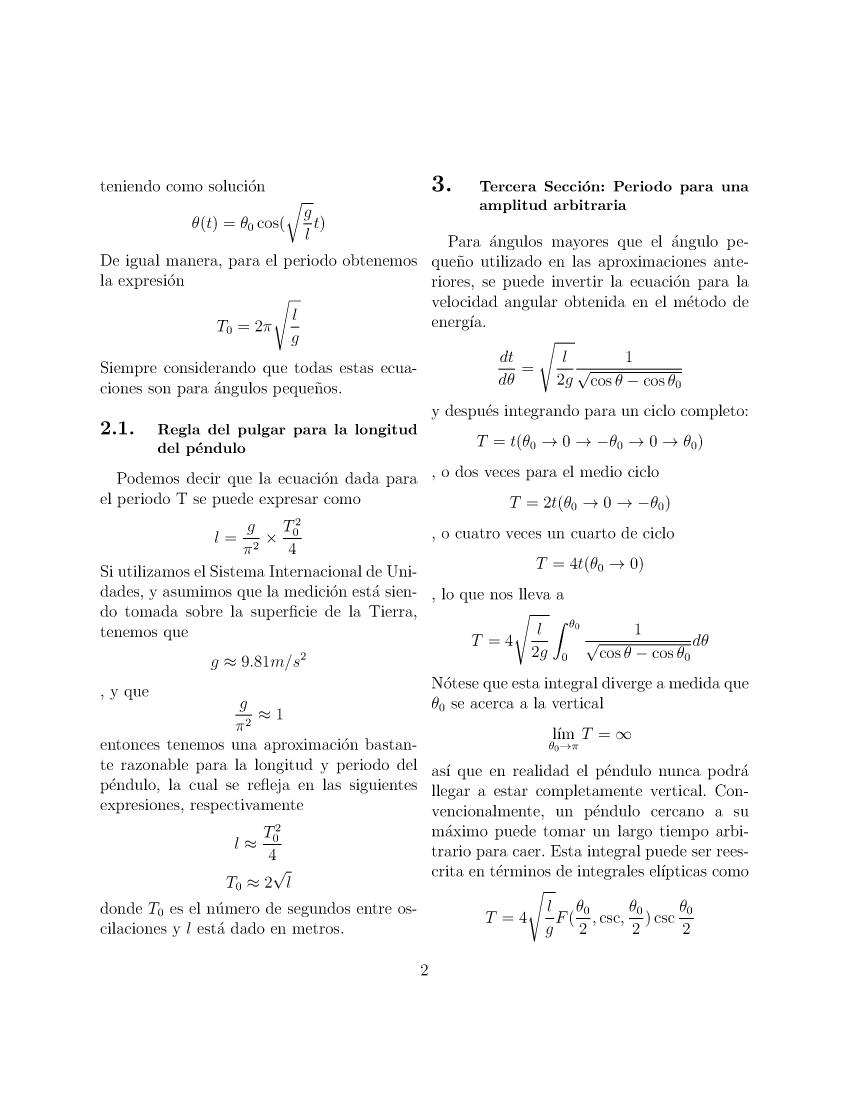
\includegraphics[width=6cm]{2}
\caption{\footnotesize Desviación de un verdadero periodo de un péndulo con ángulo pequeño.}
\end{figure}


\begin{figure}[H]
\centering
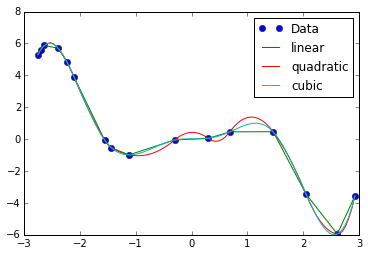
\includegraphics[width=6cm]{3}
\caption{\footnotesize Errores relativos utilizando series de potencias }
\end{figure}
\begin{thebibliography}{widestlabel}
\bibitem{w} Wikipedia, https://en.wikipedia.org/wiki/Pendulum
\end{thebibliography}

\end{document}

